\documentclass[12pt]{article} % document type and language

\usepackage{amsmath, bm, mathtools, cancel, empheq, ulem}
\usepackage{wrapfig}
%\usepackage{newtxmath} 
\usepackage[margin=1in]{geometry}
\newcommand{\pderiv}[2]{\frac{\partial#1}{\partial#2}}
\newcommand{\five}{\ \ \ \ \ }
\newcommand{\e}{\hat{\bm{e}}}
\newcommand{\curl}{\nabla\times}
\newcommand{\er}{\e_r}
\newcommand{\Div}{\nabla\cdot}
\newcommand{\phig}{\Phi_{\rm{g}}}
\newcommand{\cp}{c_{\rm{p}}}
\newcommand{\cv}{c_{\rm{v}}}
\newcommand{\ri}{r_{\rm{i}}}
\newcommand{\ro}{r_{\rm{o}}}

\newcommand{\hatt}{\hat{\bm{t}}}
\newcommand{\hatn}{\hat{\bm{n}}}
\newcommand{\hatb}{\hat{\bm{b}}}

\date{December 08, 2021}
\author{Loren Matilsky}
\title{Writing the Induction Term in Spherical Coordinates}
\begin{document}
	\maketitle
	\section{The Induction Term}
	In MHD, the evolution of magnetic field $\bm{B}$ in a fluid with local velocity $\bm{u}$ is described by
	\begin{align}
		\five\pderiv{\bm{B}}{t} = &\curl[\bm{u}\times\bm{B}-\eta\curl\bm{B}]\label{eq:ind},\\
	\text{and}\five\Div\bm{B} = &\ 0,\label{eq:divb0}
	\end{align}
which is the induction equation and ``no magnetic monopoles'' condition, respectively. Here we ignore the diffusive piece (dependent on magnetic diffusivity $\eta$) and focus on the induction term, 
\begin{align}
	\bm{I} =&\curl[\bm{u}\times\bm{B}]\label{eq:indterm}.
\end{align}
In this document, we show the various interpretations of $\bm{I}$, focusing on how it appears in spherical coordinates. 

\section{Differential Geoemetry Perspective}
We first rewrite Equation \eqref{eq:ind} (ignoring the diffusive bit, as wel will for the rest of this document) as
\begin{align}
	\five\frac{D\bm{B}}{Dt} = &\bm{B}\cdot\nabla\bm{u} - \bm{B}\Div\bm{u},\label{eq:inddg}
\end{align}
where we have expanded the product $\curl[\bm{u}\times\bm{B}]$, made use of $\Div\bm{B}=0$, and defined the material derivative (Lagrangian derivative following a fluid parcel) as $D/Dt\equiv \partial/\partial t +\bm{u}\cdot\nabla$. We examine Equation \eqref{eq:inddg} in the Frenet-Serret frame following magnetic field lines (orthogonal coordinates $\hatt$, $\hatn$, and $\hatb=\hatt\times\hatn$ as shown schematically in Figure \ref{fig:frenet}). 

\begin{wrapfigure}
	\centering
	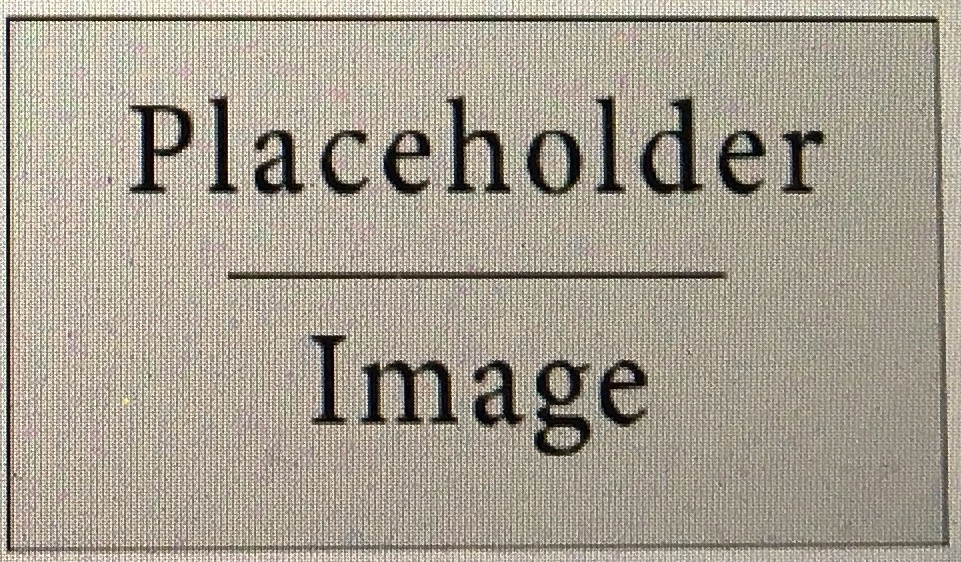
\includegraphics[width=2.5in]{placeholder.jpg}
	\caption{Temporally and spherically averaged production of poloidal magnetic energy in case M's radiative interior. The production by induction iThe y-axis is scaled logarithmically for positive and negative values away from zero. Values close to zero, in the range [-0.01, 0.01] marked by the dashed black lines, are scaled linearly.}
	\label{fig:frenet}
\end{wrapfigure}
\end{document}